\documentclass[sigconf]{acmart}
\AtBeginDocument{%
  \providecommand\BibTeX{{%
    \normalfont B\kern-0.5em{\scshape i\kern-0.25em b}\kern-0.8em\TeX}}}

\copyrightyear{2021} 
\acmYear{2021} 
\setcopyright{rightsretained} 
\settopmatter{printacmref=true}

\begin{document}
\fancyhead{}
\title{CMPT 415 - Special Research Project}
%\author{An Author}
\author{Ekamleen Maan}
\email{ekm9@sfu.ca}
\affiliation{%
  \institution{School of Computing Science\\ Simon Fraser University}
  \city{Burnaby}
  \state{BC}
  \country{Canada}
}


\begin{abstract}
This project investigates using GPT-4 to generate P4\_16 code from natural language intents for Intent-Based Networking. A closed-loop system with compiler feedback iteratively refines the code, revealing that scope-specific prompts outperform general ones for complex tasks. Results suggest LLMs can automate parts of network configuration, with reliability tied to prompt design.
\end{abstract}



\keywords{Intent Based Networking, LLMs, P4\_16, Prompts, Intent}
\maketitle
% \textbf{Start} by writing a few lines describing some background information
% \cite{ConfPaperName, ConfPaperName}, and how your work relates to the domain.  

\section{Literature Review}

Intent-Based Networking (IBN) has gained attention for its potential to abstract complex network configurations through high-level goals \cite{jain_ibn}. Several studies have explored how to formalize intents and map them to low-level control plane or data plane logic \cite{levin_ibn_survey}. However, bridging the gap between intent and programmable data planes, such as P4, remains a relatively unexplored area.

Large Language Models (LLMs) like GPT-3 and GPT-4 have recently shown promise in generating source code from natural language across multiple domains \cite{chen_codex}. These models can understand instructions and produce compilable code snippets, but their reliability varies based on prompt design and code domain complexity.

The P4 language enables fine-grained control over packet processing in the data plane \cite{bosshart_p4}, but writing correct and compilable P4 programs is non-trivial, especially for newcomers. As such, automating P4 code synthesis has practical relevance for making data plane programming more accessible.

Our work draws inspiration from the NADA project \cite{nada}, which proposed a scoped, context-specific prompt generation strategy in the domain of reinforcement learning for adaptive bitrate (ABR) video streaming. We extend this idea to programmable networks, using scoped prompts to guide GPT-4 more effectively in generating valid P4\_16 code.

This project builds on these prior insights by combining scoped prompting, compiler feedback, and closed-loop refinement into a novel application of LLMs for intent-to-P4 code synthesis.


\section{Introduction}
In traditional network configuration, operators must write and maintain low level rules and code to control packet behavior, making it error prone and inflexible. Intent Based Networking (IBN) proposes a paradigm shift: users define high level intents such as "block all HTTP traffic" or "forward packets from host A to port X" and the system handles the translation into low level configuration. This approach can reduce complexity, improve reliability, and enable more agile network management.

The growing capabilities of Large Language Models (LLMs), particularly GPT 4, offer a promising path to bridge this intent to configuration gap. In this work, we explore how GPT 4 can generate P4\_16 code, a programming language used for programming data planes, from natural language intents. By embedding the LLM within a feedback loop that uses the compiler (p4c bm2 ss) as a validator, we attempt to iteratively refine the generated code until a syntactically correct program is produced.
 

\section{Problem Definition}
Modern networks require operators to manually write low-level configurations, which is both complex and error-prone. Intent-Based Networking (IBN) aims to simplify this process by allowing users to express high-level goals in natural language. However, automatically translating these goals into correct, compilable P4\_16 programs remains a challenge.

This project explores whether a closed-loop system using large language models (LLMs), specifically GPT-4, can reliably generate and refine P4\_16 code from natural language intents. The goal is to automate the intent-to-code process with compiler feedback guiding iterative improvements.



\section{System Design}

Figure~\ref{fig:system-design}  illustrates the architecture of the closed-loop system used to translate high-level user intent into compilable P4\_16 code using GPT-4. 

The process begins with a user-provided intent in natural language. This intent is first processed by a prompt generator, which formats the input into a detailed instruction suitable for GPT-4. The language model then generates a candidate P4\_16 program based on the prompt.

The generated code is compiled using the \texttt{p4c-bm2-ss} compiler. If the code compiles successfully, it becomes a deployable P4 program. If compilation fails, the system captures the compiler errors and feeds them—along with the original prompt—back into GPT-4 to regenerate a corrected version of the program.


\begin{figure}[t]
    \centering
    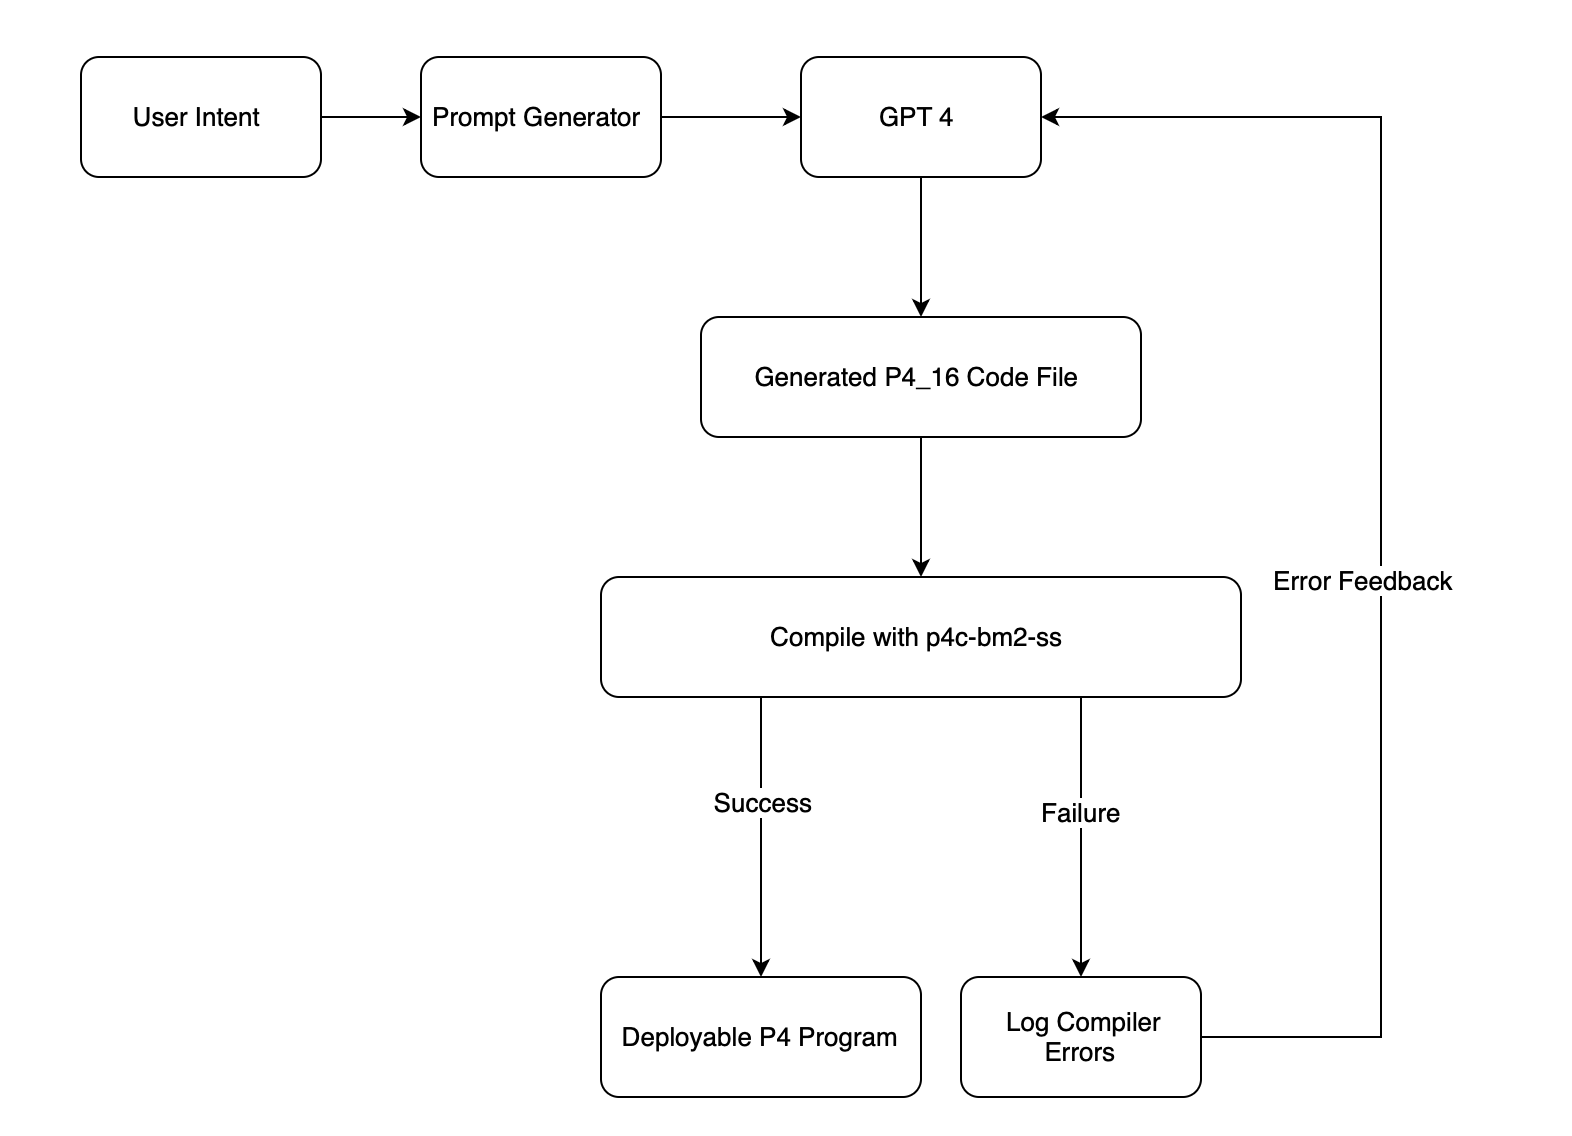
\includegraphics[width=\linewidth]{feedback_loop.png}
    \caption{Closed-loop system for intent-to-P4 compilation.}
    \label{fig:system-design}
\end{figure}



\section{Implementation}

The system is implemented using a Python script that automates the entire loop of intent translation, code generation, compilation, and correction. The steps are as follows:

\begin{enumerate}
    \item \textbf{User Input:} The user enters a high-level intent in natural language, such as ``Set source MAC to a fixed value and drop packets with destination IP 8.8.8.8''.
    
    \item \textbf{Prompt Generation:} The script transforms this intent into a detailed prompt using a predefined template designed for GPT-4.
    
    \item \textbf{Code Generation:} The prompt is sent to GPT-4 through the OpenAI API. The model responds with P4\_16 code based on the given intent.
    
    \item \textbf{Compilation:} The generated code is saved to a file and compiled using \texttt{p4c-bm2-ss}, the reference compiler for the BMv2 \texttt{v1model} architecture. If the compilation succeeds, the process ends and the code is considered deployable.
    
    \item \textbf{Error Feedback:} If the code fails to compile, the script logs the compiler error messages and asks the user whether to attempt automatic correction.
    
    \item \textbf{Fixing Errors with GPT-4:} If the user agrees, the compiler errors along with the original code are sent back to GPT-4. The model attempts to generate a corrected version of the code.
    
    \item \textbf{Retry Compilation:} The corrected code is compiled again. This process continues iteratively until the code compiles or a fixed number of iterations is reached.
    
    \item \textbf{Database Logging:} Each iteration is recorded in a local SQLite database, including the user intent, generated code, compiler output, and a success flag. This helps track progress across iterations.
\end{enumerate}

This closed-loop design allows GPT-4 to improve its output with compiler feedback, enabling more accurate translation from natural language intents to valid P4\_16 programs.

\section{Results}
This section presents the outcomes of seven experiments designed to assess the capability of GPT-4 in generating valid P4\_16 code from natural language intents, targeting the BMv2 \texttt{v1model} architecture and validated with the \texttt{p4c-bm2-ss} compiler.

\subsection*{Experiment Summary}
\begin{itemize}
    \item \textbf{Experiment 1 (Failed)}: A general prompt aimed at parsing Ethernet and IPv4 headers and forwarding packets unchanged failed after five iterations. Only one of at least four persistent errors (e.g., incomplete parser transitions) was resolved, indicating inadequate guidance for multi-header parsing.
    \item \textbf{Experiment 2 (Success)}: Simplifying the intent to parsing only Ethernet headers and forwarding packets, the same general prompt succeeded after five iterations. This suggests basic parsing tasks are more tractable with minimal refinement.
    \item \textbf{Experiment 3 (Success)}: A detailed prompt for dropping TCP packets with destination port 80 produced correct code in three iterations. The specificity of header definitions and control logic enabled rapid convergence to a compilable solution.
    \item \textbf{Experiment 4 (Failed)}: A general prompt failed to implement IPv4 packet counting per ingress port using registers, even after five iterations. Errors like incorrect register indexing persisted, revealing limitations in handling stateful operations without explicit instructions.
    \item \textbf{Experiment 5 (Success)}: A tailored prompt with precise register syntax (e.g., \texttt{register<bit<32>>(256)}) succeeded in three iterations for the same packet counting intent as Experiment 4, despite a minor compiler warning (e.g., unused variable). This highlights the value of scope-specific guidance.
    \item \textbf{Experiment 6 (Success)}: A scoped prompt for header modification intents—rewriting destination IP (10.0.0.1 to 10.0.0.2), NAT translation (192.168.0.100 to 172.16.0.100), and setting a fixed source MAC with dropping for IP 8.8.8.8—succeeded with an average of 4.67 iterations (min: 2, max: 9). This demonstrates flexibility across related tasks with proper scoping.
    \item \textbf{Experiment 7 (Failed)}: A general prompt again failed to implement register-based IPv4 packet counting after ten iterations, with errors such as mismatched bit-widths persisting. This reinforces the need for detailed, intent-specific prompts for advanced functionality.
\end{itemize}

\subsection*{Quantitative Analysis}
The system achieved a success rate of 57.1\% (4 out of 7 experiments succeeded). For successful cases:
\begin{itemize}
    \item Average iterations to success: 4.25 (Experiment 2: 5, Experiment 3: 3, Experiment 5: 3, Experiment 6: 4.67 average across three intents).
    \item Minimum iterations: 2 (Experiment 6, Intent: Set source MAC to a fixed value and drop the packet if the destination IP is 8.8.8.8).
    \item Maximum iterations: 9 (Experiment 6, Intent: Rewrite destination IP to 10.0.0.2 if it is 10.0.0.1).
\end{itemize}
For failed cases:
\begin{itemize}
    \item Average iterations attempted: 6.67 (Experiment 1: 5, Experiment 4: 5, Experiment 7: 10).
    \item Maximum iterations: 10 (Experiment 7), with no success.
\end{itemize}

Notably, iteration counts did not always align with perceived intent complexity. Easier intents like parsing (Experiment 2, 5 iterations) and filtering (Experiment 3, 3 iterations) succeeded within 3–5 iterations, and the register-based intent in Experiment 5 took 3 iterations with a tailored prompt. However, in Experiment 6, the seemingly complex intent of setting a source MAC and dropping packets (2 iterations) converged faster than the simpler IP rewriting intent (9 iterations). Failed cases with complex intents (Experiments 1, 4, 7) averaged higher iterations (6.67), suggesting that while complexity can increase iterations, prompt design and LLM variability also play significant roles in efficiency.

\subsection*{Key Insights}
\begin{itemize}
    \item \textbf{Prompt Specificity Drives Success}: General prompts consistently failed for complex intents (Experiments 1, 4, 7), while scope-specific prompts succeeded (Experiments 3, 5, 6), reducing iterations and errors by providing clear semantic guidance.
    \item \textbf{Task Complexity Impacts Feasibility}: Simple stateless tasks like header parsing (Experiment 2) and TCP filtering (Experiment 3) succeeded with fewer iterations, whereas stateful operations like register counting (Experiments 4, 7) failed without precise instructions.
    \item \textbf{Compiler Feedback Has Limits}: The feedback loop corrected syntactic issues (e.g., one error in Experiment 1 after five iterations), but could not overcome semantic gaps in general prompts, as seen in the persistent failures of Experiments 4 and 7.
    \item \textbf{Advanced Features Need Explicit Guidance}: Register-based logic succeeded only with detailed syntax and scoping (Experiment 5), unlike header parsing or forwarding, which worked with minimal prompts (Experiments 2, 3).
    \item \textbf{Scope-Based Prompting Enhances Reliability}: Inspired by the NADA project’s context-driven design separation, structuring prompts by functionality (e.g., parsing, modification) improved outcomes across diverse intents, as evidenced by Experiment 6’s success with an average of 4.67 iterations.
\end{itemize}

These findings validate the hypothesis that effective prompt engineering in intent-based networking hinges on aligning prompts with the functional scope of the intent. General prompts suffice for basic tasks, but moderately complex intents demand tailored, domain-specific instructions. Future enhancements could leverage intent classifiers or scope mappers to automate prompt selection, streamlining the translation process.

\section{Conclusion and Future Work}

This project explored how Large Language Models, specifically GPT-4, can be used to generate P4\_16 code from high-level natural language intents. We implemented a closed-loop system that iteratively refines the code based on compiler feedback until a valid program is produced. Through a series of experiments, we found that while general prompts work for simple parsing and forwarding tasks, scope-specific prompt templates significantly improve success rates for moderately complex intents such as header modification or register usage.

Inspired by the NADA project, we adopted a scope-based approach to prompt generation and demonstrated its effectiveness across a variety of networking use cases. Our findings suggest that LLMs have the potential to assist in intent-to-configuration translation, but reliability depends heavily on how well the prompt aligns with the underlying intent.

While the findings are promising, they are based on a limited set of nine experiments and should be interpreted as exploratory rather than conclusive. Further large-scale testing is required to strengthen the statistical validity of the results.

Future work could focus on several directions. One possibility is to develop a classifier that automatically identifies the intent scope and selects the appropriate prompt template. Another is to fine-tune LLMs on a corpus of syntactically valid P4\_16 code to improve reliability. Additionally, integrating formal verification or behavioral testing into the feedback loop may allow not just syntactic correctness, but also semantic validation. 



\bibliographystyle{ACM-Reference-Format}
\bibliography{ref}
\end{document}